
\glsresetall
\section{Introduction}
    As more of society becomes integrated with \gls{ml}, bias, fairness, and the formalization of \gls{ml} standards attract more attention~\cite{10.1007/978-3-030-13469-3_68, anne2018women, wang2018racial}. Thus, an effect of the growing dependency on \gls{ml} are growing concerns for biased and unfair algorithms, \eg untrustworthy and racist \gls{fr} systems~\cite{england2019,snow2018}.
    


    Typically, \glspl{cnn} are trained on faces identified by a detection system. Specifically, for \gls{fr}, the goal is to encode faces in an N-dimensional space such that samples of the same identity are neighbors and those of different identity of further apart. Thus, the goal is to identify subjects with face encodings. We can deploy a \gls{cnn} to encode faces, and then compare via a similarity score: assume pairs with a high enough score are \emph{genuine}; else, an \emph{imposter}. 

\begin{figure}
    \centering
    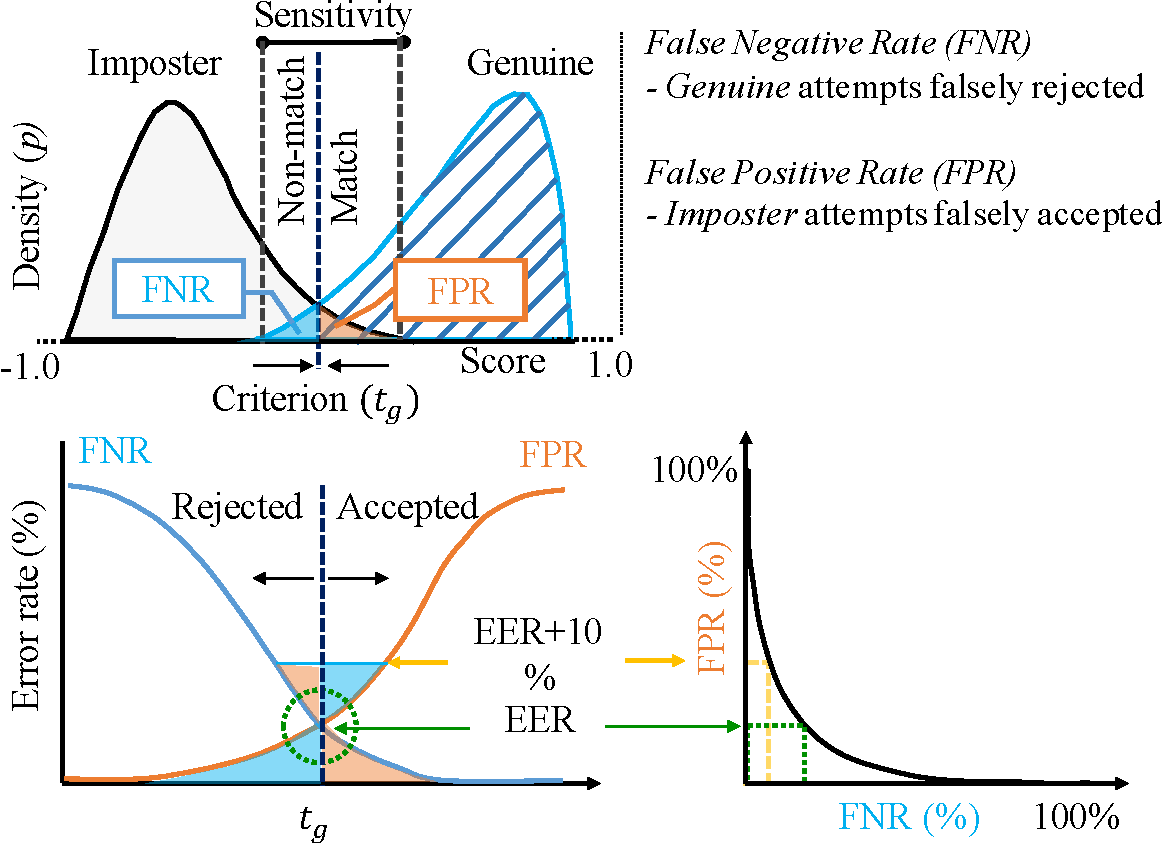
\includegraphics[width=\linewidth]{figures/fig1-crop.pdf}
    \caption{\small{\textbf{Depiction of biometrics.} The \gls{sdm} (\emph{top-left}) shows the sensitivity related to a single threshold $t_g$. Translated to error rate (\emph{bottom-left}), a direct trade-off between FNP and FPR. In practice, this is entirely application dependent. Specifically, the specific chose in desired FPR (\%) (\emph{bottom-right}).}}
    \label{fig:biometrics}
\end{figure}
    % \begin{figure}[t!]
    %     \centering
    %     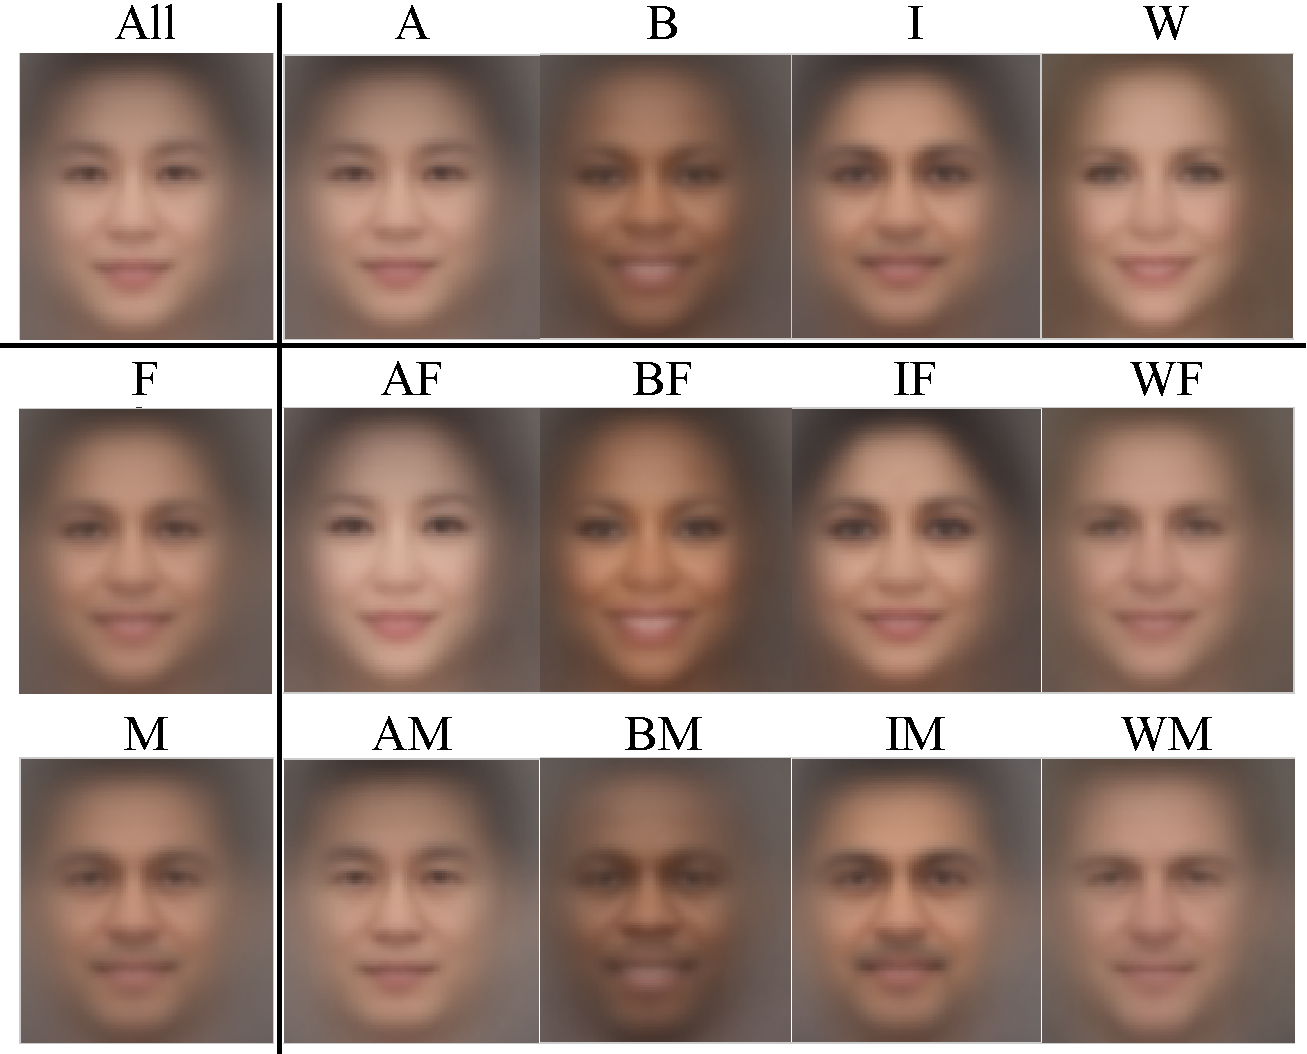
\includegraphics[width=.8\linewidth]{figures/montage.pdf}
    %     \caption{\small{\textbf{\gls{bfw}.} Average face of the different subsets: \emph{top-left}: the entire \gls{bfw}; \emph{top-row} per race;  \emph{left-column}: per gender. The others represent the ethnicity and gender of the race and gender, respectively. Table~\ref{tab:ethnic-splits} defines the acronyms of subgroups.}}
    %     \label{fig:avg-faces}
    % \end{figure}
    
    When comparing scores, typically, a fixed threshold sets the decision boundary (Fig.~\ref{fig:biometrics}). Thus, features of the same identity must satisfy a criterion via a single value~\cite{deng2019arcface, liu2017sphereface, wang2018additive, wang2018cosface}. However, we found that a single (\ie global) threshold is a crude measure that leads to skewed errors - the held-out set used to determine the threshold tends to share the same distribution with the test data, which favors specific demographics that are a majority. That skew, the difference in the performance of an algorithm of certain demographics, is our definition of bias. A key question is: \emph{is \gls{fr} too biased, or not?} 
    

\begin{table*}[!t]
    \centering
    \caption{\small{\textbf{Database stats and nomenclature, optimal thresholds ($t_o$), and accuracy scores.} \textit{Header:} Subgroup definitions. \textit{Top:} Statistics of \gls{bfw}. \textit{Bottom::} Number of pairs for each partition. Columns grouped by race and then further split by gender. Out of millions of pairs, accuracy is inconsistent across subgroups. Furthermore, $F$ tends to perform inferior to that of $M$ for all but B.}}\label{tab:ethnic-splits}
    \scalebox{.75}{
     \resizebox{\textwidth}{!}{%
    \begin{tabular}{r c c c c c c c c l}
        \toprule
        & \multicolumn{2}{c}{Asian (A)} & \multicolumn{2}{c}{Black (B)}  & \multicolumn{2}{c}{Indian (I)}& \multicolumn{2}{c}{White (W)}\\
        \cmidrule(l){2-3} \cmidrule(l){4-5} \cmidrule(l){6-7}\cmidrule(l){8-9} % spanning less than the full width of the table - you can add (r) or (l) just before the opening curly bracket to shorten the rule on the left or right side
         & Female (AF) & Male (AM) & BF & BM& IF & IM & WF & WM&Aggregated\\ % Column names row
        \midrule

       \# Faces  &  2,500&  2,500& 2,500 & 2,500& 2,500 & 2,500 & 2,500 & 2,500 &20,000 \\ % row 1
        \# Subjects & 100& 100& 100  & 100  & 100  & 100& 100 &100&800  \\ % row 2
        \# Faces / Subject  & 25 & 25    & 25 & 25 & 25  & 25  &  25 & 25 & 25\\ % row 3
        % \midrule
\specialrule{.01em}{.05em}{.05em}
            \# Positive Pairs &  30,000&  30,000& 30,000 &30,000 & 30,000 &30,000&30,000 & 30,000 &240,000 \\ % row 1
        \# Negative Pairs & 85,135&  85,232& 85,016  & 85,141  & 85,287  & 85,152& 85,223 &85,193&681,379  \\ % row 2

        \# Pairs (Total) & 115,135 & 115,232    &115016 &115,141 & 115287  & 115,152  &  115,223& 115193 & 921,379\\ % row 3
        % \midrule
        % \specialrule{.01em}{.05em}{.05em}
        % Acc$@t_g$ & 0.941 & 0.952  & 0.967 & 0.960 & 0.958 &0.962  & 0.973 & 0.981 &0.962 $\pm$0.012 \\
        % $t_o$ & 0.255 &  0.246 & 0.277 &0.242  &0.297 & 0.264& 0.233 &0.239 &0.257$\pm$0.006\\ % row 4
        
        % Acc$@t_o$ & 0.942 &0.952 &0.968 &0.961 &0.960 &0.962 & 0.974 &0.982 & 0.963 $\pm$ 0.012\\
        \bottomrule
    \end{tabular}}
    % \glsunset{af}
    }
    % % \glsunset{af}
    % \glsunset{am}
    % \glsunset{bf}
    % \glsunset{bm}
    % \glsunset{if}
    % \glsunset{im}
    % \glsunset{wf}
    % \glsunset{wm}
    % \vspace{-12pt}
\end{table*}

    
    Making matters more challenging is that race and ethnicity are loosely defined. For example, the US Census Bureau allows an individual to self-identify race.\footnote{\scriptsize\href{https://www.census.gov/mso/www/training/pdf/race-ethnicity-onepager.pdf}{www.census.gov/mso/www/training/pdf/race-ethnicity-onepager}} For this work, we define subgroups as specific sub-populations with face characteristics similar to those found in a region. 
    
    
    The adverse effects of a global threshold are two-fold: \textbf{(1)} the mapping produced by a \gls{cnn} is nonuniform. Therefore, distances between pairs of faces in different demographics vary in distribution of similarity scores (Fig~\ref{fig:detection-model}); \textbf{(2)} the evaluation set is imbalanced as well. Particular demographics making up a majority of the population will carry most weight on the reported performance ratings. Reported results favor the common traits over the underrepresented. Alas, demographics like gender, ethnicity, race, and age are underrepresented in most public datasets~\cite{merler2019diversity, wang2018racial}. 
    
    % The result is various types of biases in FR systems in favor of or against particular demographics remain a question.
    
    For \textbf{(1)} we propose subgroup-specific (\ie optimal) thresholds; to address \textbf{(2)}, we introduce a new benchmark for measuring bias in \gls{fr}, \gls{bfw} (Table~\ref{tab:compared} \&~\ref{tab:ethnic-splits}). \gls{bfw} allows for a fair evaluation of \gls{fr} systems, while enabling demographic-specific ratings to be reported. We use \gls{bfw} to gain a deeper understanding of the extent of bias present in \gls{soa} \gls{cnn} used to encode faces. Then, we suggest a mechanism to mitigate problems of bias with more balanced performance ratings for different demographics. Specifically, we propose using an adaptive threshold that varies depending on the characteristics of detected facial attributes (\ie gender and ethnicity, Fig~\ref{fig:avg-faces}). We show an increase in accuracy with a balanced performance for different subgroups. Similarly, we show a positive effect of adjusting the similarity threshold based on the facial features of matched faces. Thus, selective use of similarity thresholds in current \gls{soa} \gls{fr} systems provides more intuition in \gls{fr} research with a method easy to adopt in practice. 
    
    
    The contributions of this work are 3-fold. (1) We built a balanced dataset as a proxy to measure verification performance per subgroup for studies of bias in \gls{fr}. (2) We revealed an unwanted bias in scores of face pairs - a bias that causes ratings to skew across demographics. For this, we showed that an adaptive threshold per subgroup balances performance (\ie the typical use of a global threshold unfavorable, which we address via optimal thresholds). (3) We surveyed humans to demonstrate bias in human perception (NIH-certified, \textit{Protect Humans in Research}).%\footnote{NIH-certified, \textit{Protect Humans in Research}.}%19-09-08}.}
    % \begin{enumerate}
    %     \item Built a balanced dataset as a proxy to measure verification performance per subgroup.
    %     \item Analyzed an unwanted bias in scores of face pairs while showing that optimal thresholds determined per subgroup significantly boost and balance performances.
    %     \item Showed bias causes inconsistencies in ratings across demographics-- the typical use of a global threshold unfavorable. We mitigate the problem via adaptive thresholds.
    %     \item Conducted human-evaluations to demonstrate bias in human perception.\footnote{NIH-certified, \textit{Protect Humans in Research}, \textcolor{red}{IRB 19-09-08}.}
    % \end{enumerate}
